\documentclass[10pt,a4paper]{article}
%----------packages---------------
\usepackage[utf8]{inputenc}
\usepackage{amsmath}
\usepackage{amsfonts}
\usepackage{amssymb}
\usepackage{amsmath}
\usepackage{graphicx}
\usepackage{floatflt}
\usepackage[left=1.5cm,top=0.8cm,right=2.5cm,bottom=0cm,bindingoffset=0.5cm]{geometry}
%----------end of packages---------
\setlength{\parindent}{0pt}
\author{Dominik Kesim, Magnus Specht, Sebastian Paule,}
\pagestyle{plain}
\begin{document}
\begin{floatingfigure}[r]{0.03\textwidth}
\centering
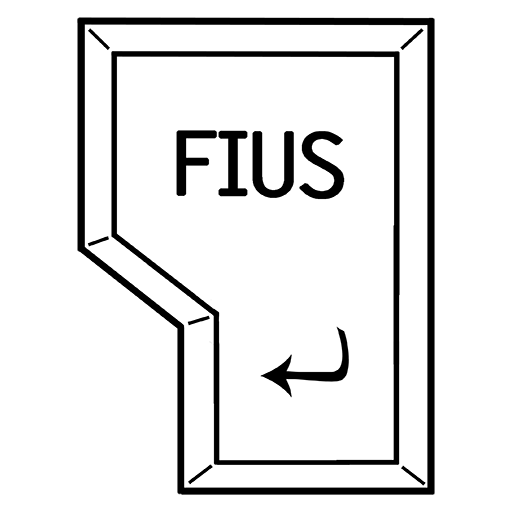
\includegraphics[width=0.05\textwidth]{fius-logo.png}
\end{floatingfigure}
\vspace{-1cm}
\textbf{Vorlesungsumfrage der Fachgruppe Informatik - Ergebnisse}

\vspace{0.3cm}
\line(2,0){480} \\

Sehr geehrte Dozenten,\\
anbei erhalten sie die Auswertung der Vorlesungsumfage, die sie vor kurzem in ihrer Veranstaltung durchgeführt haben.
\\
Ihre Fachgruppe Informatik\\

\vspace{2pt}
\line(2,0){480}
\vspace{2pt}\\

\textbf{Achtung:} Dieser Bogen wurde nicht zentral von der Universität Stuttgart ausgewertet, sondern von der Fachgruppe Informatik (FIUS).\\

\textbf{Veranstaltung:}\hspace{0.1cm}
%# print next data #%
\\
\textbf{Dozent:}\hspace{0.2cm}
%# print next data #%

\vspace{2pt}
\line(2,0){480}
\vspace{2pt}\\

\begin{enumerate}
	%# for children #%
	\item
	%# print data #%
	
    \begin{itemize}
    	\setlength\itemsep{1em}
        %# for children #%
    	\item[]
		%# print data #%
        %# end for #%
    \end{itemize}
	
	\vspace{2pt}
	\line(2,0){480}
	\vspace{2pt}\\
    %# end for #%
\end{enumerate}

\end{document}\textsl{•}